% THIS IS SIGPROC-SP.TEX - VERSION 3.1
% WORKS WITH V3.2SP OF ACM_PROC_ARTICLE-SP.CLS
% APRIL 2009
%
% It is an example file showing how to use the 'acm_proc_article-sp.cls' V3.2SP
% LaTeX2e document class file for Conference Proceedings submissions.
% ----------------------------------------------------------------------------------------------------------------
% This .tex file (and associated .cls V3.2SP) *DOES NOT* produce:
%       1) The Permission Statement
%       2) The Conference (location) Info information
%       3) The Copyright Line with ACM data
%       4) Page numbering
% ---------------------------------------------------------------------------------------------------------------
% It is an example which *does* use the .bib file (from which the .bbl file
% is produced).
% REMEMBER HOWEVER: After having produced the .bbl file,
% and prior to final submission,
% you need to 'insert'  your .bbl file into your source .tex file so as to provide
% ONE 'self-contained' source file.
%
% Questions regarding SIGS should be sent to
% Adrienne Griscti ---> griscti@acm.org
%
% Questions/suggestions regarding the guidelines, .tex and .cls files, etc. to
% Gerald Murray ---> murray@hq.acm.org
%
% For tracking purposes - this is V3.1SP - APRIL 2009

\documentclass{proseminar}
\usepackage[hidelinks]{hyperref}
\usepackage{graphicx}

\begin{document}

\conferenceinfo{Albert-Ludwigs Universit\"at Freiburg\\Technische Fakult\"at, Institut f\"ur Informatik\\Lehrstuhl f\"ur Datenbanken \& Informationssysteme}{}

\title{Abusive behavior in social media}

\numberofauthors{1}
\author{
Tarek Saier\\
\email{tareksaier@gmail.com}
}

\maketitle

\section{Introduction}
Usage of online platforms of all shapes and sizes nowadays is a common part of may people's everyday life. Just like human interaction offline, user interaction on Facebook, Twitter, online forums etc. is not always positive. For all the good like helpful contributions to Wikipedia and engaged discussion on reddit, there also is abusive behavior taking place.

While the seriousness of the effects such behavior can have on victims may have been downplayed in earlier days of the web, it is clearly as a serious problem. Furthermore, with the media reporting on large social networks failing to control abusive behavior and thus influencing their public image, it is in the financial interest of companies running such networks to detect and remove or, if possible, even prevent such behavior.

This report will give an introduction into the topic of \emph{Abusive behavior in social media} --- or more precise: the decection of such behavior --- and is structured as follows. Section 2 will give a wider view on the topic, provide necessary background information and shortly describe approaches for trackling the problem at hand. In section 3 the focus will be put on machine learning as one possible approach. While giving a short overview of the steps of a machine learning procedure in general, noteworthy particularities with regards to abusive behavior in social media will be explained. Section 4 will introduce two concrete approaches --- efforts for detecting abusive comments on Yahoo! on the one hand and agressive Twitter accounts on the other. This will be followed by a comparison of the two. Lastly, section 5 will conclude the report.

\section{Background}
In the physical world, abusive behavior can take many forms. Acts of bullying, for example, can be categorized into four types: physical, verbal, relational and damage to property\cite{bullying:2014}. In social media, physical abuse is not possible and damage to property at least rather unlikely and certainly not commonplace. While relational bullying is a possiblity, this report will focus on verbal types of abusive behavior in social media from hereon. Put simply, the remainder of this report is concerned with detecting absusive or malicious intent in text based communication.

\subsection{Problem formulation}
On a high level of abstraction, the task at hand is detecting and stopping abusive behavior in a social media setting. Within the scope of this report \emph{''behavior''} boils down to communication in text form. This communication may be associated with user accounts. User accounts in turn also may have different qualities of interest.

Looking at it from the perspective of an entity operating a social platform, the problem can be formulated as: given all the information about the actors on our platform and the communication they engage in, how can abusive communication be detected? Depending on what constitues an actor on a platform, different possibilities for approaching that goal exist. For example, in the case of platform that wants its user accounts to be as representative of the real person controlling the account as possible (e.g. Facebook), it might be viable to detect abusive \emph{accounts} in order to stop abusive communication. On the other hand, for a platform where the notion of an account does not hold much informational value, it might be more feasable to try and detect abusive communication from its contents only. Examples for the latter setting might be online comment sections that allow anonymous posting, or platforms like 2channel\footnote{\url{http://2ch.net/}} or 4chan\footnote{\url{https://www.4chan.org/}} that just give each participant an ID, so messages of the same origin can be identified as such, while connecting from a different IP address results in a different ID and the traceability of a common origin of messages is lost.

\subsection{Challenges}
As just described, the amount of information available can pose a challenge for detecting abusive behavior and render certain approaches nonviable. Aside from the mentioned feasablility to model user accounts, brevity of communication (e.g. on Twitter due to its 140 character limit) can also pose a hurdle.

Another set of challanges is given by the fact that the communication to be examined happens in natural language from the hands of humans. This means for example that:
\begin{itemize}
\item Offensive language may intentionally be obfuscated (e.g. \emph{ni9 9er}) rendering simple keyword matching ineffective.
\item Some language might be acceptable within one group of people but offensive within another.
\item The offensive nature of an utterance might only come to light when considering a larger context (e.g. multiple sentences) while its parts taken out of context are harmless.
\item Sarcasm might falsely be detected as abusive language, while constant sarcasm towards a user could also be a form of bullying.
\item Language changing over time might require detection methods to be adapted over and over again.
\end{itemize}

Lastly, advancing the field of abusive behavior detection can be challenging because a lot of work may target different types of abusive behavior (e.g. bullying, aggression, hate speech, derogatory language, profanity) and therefore be incompatible.


\subsection{Approaches for solving the problem}
The following will give a very brief overview of some approaches to detect abusive language, while the remainder of the report will focus on machine learning as one such approach.

\subsubsection{Most basic} An overly simplistic approach --- nevertheless often seen applied in online forums --- is to maintain a list of words that are deemed offensive, and filtering out those words or messages containing at least one blacklisted word. As described before this is easily circumvented by users that intentionally misspell or obfuscate offensive terms. Another problem with this approach is that a lot of harmless words containing offensive terms (e.g. to snigger) might falsely be flagged.

\subsubsection{More sophisticated} More sophisticated approaches don't just take into account the words as isolated merely syntactical bits of information. They rather bring them into context and try to evaluate them semantically. A first step in this direction is, for example, considering the TFIDF scores of words. Furthermore, to allow for variations and obfuscated versions of words, not the words themselves but n-grams can be used\cite{Yin:2009}. Recent techniques most often are machine learning\cite{Yahoo:2016}\cite{Twitter:2017} or deep learning\cite{DeepLearning:2017} approaches that take into account many different language-based, network-based and, if appilcable, user-based features.

\section{Machine learning}
To develop a supervised machine learning approach for the task of abusive behavior detection one needs to:
\begin{itemize}
\item have or produce a data set with labels (e.g. a large set of messages labeled \emph{abusive} or \emph{not abusive})
\item decide on which features to extract from the data
\item decide on a learning algorithm
\item evaluate the system
\end{itemize}
The following sections will briefly describe each step and, if appilcable, highlight noteworthy particularities with regards to abusive behavior in social media.

\subsection{Data collection}
For the algorithm to work on, a large set of labeled data is necessary. This can be freely available and established testing sets (like the MovieLens data set\footnote{\url{https://grouplens.org/datasets/movielens/}} for the movie domain) or newly obtained data labeled via crowdsourcing or trained personnel. The data will be used to train and also evaluate the system.

In the case of abusive behavior detection in social media, data is still problematic to a certain extend, since there is no de facto standard testing set for abusive language\cite{Yahoo:2016}.

\subsection{Feature extraction}
The extraction of features from the data is essential in that it dictates what the learning algorithm gets as its input. This step might include \emph{feature processing} steps --- for example the generation of n-grams from whole words.

Common features in the case of abusive behavior detection in social media are text- or language-based (e.g. n-grams, results of seniment analysis and word embeddings), network-based (e.g. cliques and centrality scores) and user-based (e.g. account creation and activity times).

\subsection{Learning}
Once a labeled data set and its features are available, a learning algorithm can be trained with it to afterwards itself attempt to put correct labels on data.

\subsection{Evaluation}
The last step is to use the trained model for predicting labels and checking these predictions against the true labels. This ties in with the data collection step, which means for abusive behavior detection in social media the \emph{creation} of a set with ''true'' labels from scratch is most propably necessary which makes the comparison of evaluation results of different approaches difficult.

\section{Two concrete approaches}
The basis of this report are two papers, \emph{Abusive Language Detection in Online User Content} by Nobata et al.\cite{Yahoo:2016} and \emph{Mean birds: Detecting Aggression and Bullying on Twitter} by Chatzakou et al.\cite{Twitter:2017}. Sections 4.1 and 4.2 will describe and discuss them respectively and section 4.3 will compare the two.

\subsection{Abusive Yahoo! comments}
\subsubsection{Task}
In \cite{Yahoo:2016} Nobata et al. set out to detect comments on Yahoo! News\footnote{\url{https://www.yahoo.com/news/}} and Yahoo! Finance\footnote{\url{https://finance.yahoo.com/}} that contain hate speech, derogatory language or profanity. For their definitions and examples of the three categories see Figure \ref{fig:yahoo_hate_speech}.

\begin{figure*}
\centering
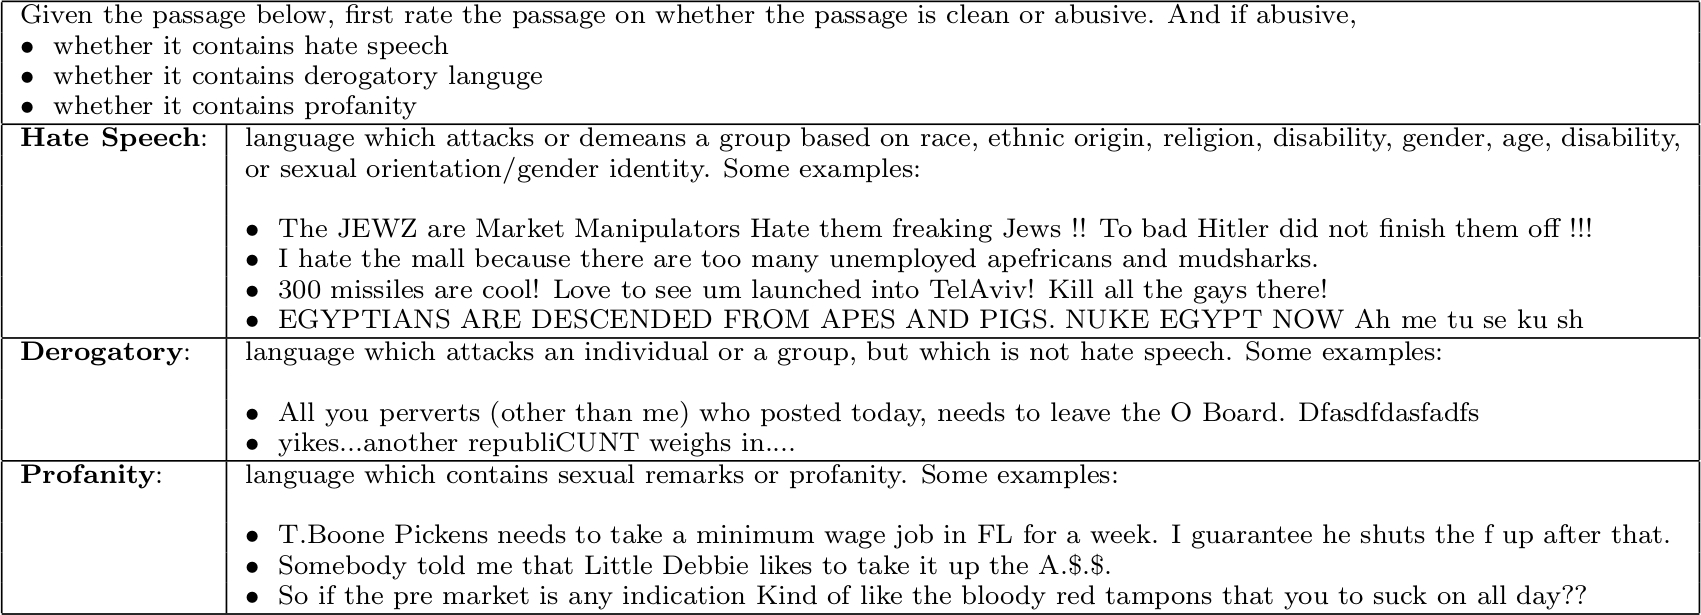
\includegraphics[width=\textwidth]{img/yahoo_hate_speech}
\caption{Outline of annotation instructions given to Yahoo! employees for labeling comments in \cite{Yahoo:2016}.}
\label{fig:yahoo_hate_speech}
\end{figure*}

\subsubsection{Method}
\paragraph{Data} The data sets are based on comments from Yahoo! News and Yahoo! Finance. In total 4 different sets are used. The first of these, the \emph{primary data set} is comprised of a random 10\% of the comments from the time between October 2012 and January 2014, plus all comments that have been reported as abusive by users during that time. In total there are a little over 2.1 million comments of which about 13\% are labeled as abusive. For training and testing the data is split into parts of 80\% and 20\% respectively. Second, the \emph{temporal data set} is sampled between April 2014 and April 2015. It consists of about 1.2 million comments of which a little over 7\%\footnote{According to the authors the significantly lower number compared to the \emph{primary data set} is explained by the fact that their models were already in use on the platforms during that time.} are labeled abusive. The \emph{WWW2015 data set} is taken from a prior work were the comments are only taken from Yahoo! Finance during an unspecified 6 month period. There are almost 1 million comments, about 6\% of which are labeled abusive. Lastly, the \emph{evaluation data set}, a data set where extra effort was put into a valid labeling, is sampled and selected between March and April of 2015 and consists of 1000 clean and 1000 abusive comments.

\paragraph{Labelling}
For labelling the comments Nobata et al. rely on Yahoo! employees which already were used to text annotation tasks and also received training specifically for the judgment guidelines outlined in Figure \ref{fig:yahoo_hate_speech}. When multiple employees were given the same comments to label (which was done for abovementioned \emph{evaluation data set} where each comment was labelled by 3 people) their agreement rate was 0.922 and the Fleiss's kappa 0.843 concerning the clean or abusive dichotomy. When looking at the more fine grained distiction between hate speech, derogatory language and profanity the agreement rate is 0.603 and Fleiss's kappa 0.456.

For comparison Nobota et al. also looked at the results of untrained raters via Amazon's Mechanical Turk\footnote{\url{https://www.mturk.com/}}. Workers were allowed to label at most 50 comments and were provided with the guidelines shown in Figure \ref{fig:yahoo_hate_speech}. Labels gathered in this manner resulted in an agreement rate of 0.867 and a Fleiss's kappa of 0.401. For the fine-grained distiction the values drop to 0.405 and 0.213 respectively.

\paragraph{Feature extraction} The features used in \cite{Yahoo:2016} are grouped into 4 classes: n-grams, syntatic, linguistic and distributional semantics. The \emph{n-grams} used are generated from not normalized text and from 3 to 5 characters long. By not normalizing the text from which the n-grams are generated the authors hope to model spelling variations of offensive words. To capture dependencies between words that n-grams can't, \emph{syntactic} features derived from ClearNLP\footnote{\url{http://clearnlp.wikispaces.com/}, since February 2016 succeeded by the NLP4J project: \url{https://emorynlp.github.io/nlp4j/}} are used. These encompass Part-of-speech tags (e.g. if a word is a pronoun or interjection, etc.) and dependency relations between words. \emph{Linguistic} features include many basic things like the average length of words or the number of URLs, but also more abstract notions like the number of words associated with hate speech (based on Hatebase\footnote{\url{https://www.hatebase.org/}}) and the number of discourse connectives (based on \cite{Pitler:2009}). Lastly, \emph{distributional semantics} features are divided into two sets of features based on word embeddings and one set of features based on comment embeddings. These features model the context of words or whole comments respectively. Put simply, in the case of a word, its embedding may be used to detect words with similar meaning, since words with similar meaning are used in similar contexts.

% \cite{Distributed:2014}

\paragraph{Machine learning} In their experiments Nobata et al. ''use Vowpal Wabbit's\footnote{\url{http://hunch.net/~vw/}} regression model in its standard setting with a bit rate of 28''\cite{Yahoo:2016} for learning and prediction. Experiments are performed for each of the data sets described in the beginnig of this seciton. Their results are described in the follwing section.

\subsubsection{Results}
For the \emph{primary data set} the usage of all features yields the best results (an F-score of 0.795 for Yahoo! Finance and 0.817 for Yahoo! News). Using just token n-grams\footnote{In natural language processing a token is a meaningful element (e.g. a word or phrase).} or character n-grams, however, leads to results that are almost as good (Finance=0.772, News=0.740 and Finance=0.726, News=0.769 respectively).

Predictions for the \emph{WWW2015 data set} (as mentioned before this data set only contains comments from Yahoo! Finance) also are best if all features are used (F-score 0.783) and outperform the research the data was initially used in\cite{Yahoo:2015} (AUC 0.9055 and 0.8007 respectively). In fact, token n-grams, character n-grams and two of the distributional semantics feature classes each taken separately also outperform the approach from 2015.

The \emph{evaluation data set} is used to see how different ways of processing the 3 given labels effect the prediction results. The predictions perform best with respect to comments where all labelers agreed (F-score 0.839) followed by measuring predictions against the majority of labels given (F-score 0.826). Comparatively low performance results when using those labels where exactly 2 out of 3 raters agreed (F-score 0.431).

For experiments with the \emph{temporal data set} it is split into slices of 20k comments each. Then the following experiments are run:
\begin{itemize}
\item \lbrack Original\rbrack\\train on the \emph{primary data set}, predict for slice \texttt{t}
\item \lbrack Each Slice\rbrack\\train on slice \texttt{t}, predict for slice \texttt{t+1}
\item \lbrack Accumulated\rbrack\\train on slices \texttt{(0..t)}, predict for slice \texttt{t+1}
\end{itemize}

The results are shown in Figure \ref{fig:yahoo_temporal}. The fact that the results for Accumulated are better than those for Original indicates that it is more important to have a recent training set than to have a large one. In other words, the proposed model is likely sensitive to language changing over time. Furthermore, the fact that the results for Accumulated only show a remarkable upwards trend for the first few slices, shows that a reasonably good effort for detecting abusive content can be realized with comparatively small training data.

\begin{figure}
\centering
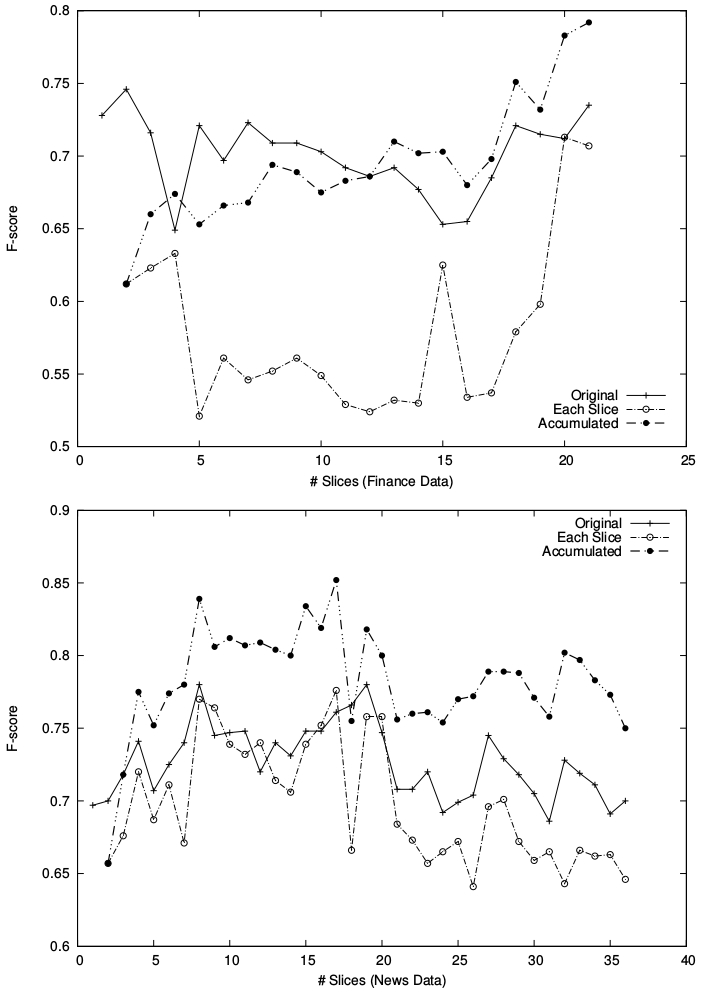
\includegraphics[width=0.45\textwidth]{img/yahoo_temporal}
\caption{Temporal evaluations in \cite{Yahoo:2016}.}
\label{fig:yahoo_temporal}
\end{figure}

\subsubsection{Discussion}
Nobata et al. present a very thorough examination of their topic. They test their model on different data sets, compare it to previous approaches and show the influence of all the types of features they chose to use. It is nice to see that a combination of all the features they extracted gives the best results. Additional experiments like the comparison between trained in-house staff and crowdsourcing workers as well as the testing of different gold standard references on the \emph{evaluation data set} allow for interesting insights.

In their evaluation of the classifier on the \emph{evaluation data set} it would, although it is not the main point, be interesting to know which data set was used for training. Since the set is orders of magnitude smaller than the other sets it can be assumed it wasn't split into a training and test set. This ties into a remark concerning them making the \emph{evaluation data set} freely accessible. It surely is a step forward since other approaches can be tested with regards to their results in classifying the set, but their can be no direct comparison of competing models insofar as the training data will be different.

As mentioned in the conclusion of the paper, it would be interesting to see how the approach works with other languages. Especially languages that don't use latin script would be of interest. Also, as mentioned by the authors, the additional integration of conext (e.g. surrounding comments, user profiles, etc.) seems woth looking into.
%- mentions outperforming ''state of the art deep learning approach'': outperforms approach based (soley?) on word2vec (which is deep learning), also uses word2vec\\

\subsection{Aggressive Twitter accounts}
\subsubsection{Task}
In \cite{Twitter:2017} Chatzakou et al. make an approach to detect Twitter accounts that conduct bullying or aggressive behaviour. They define the terms as shown in Figure \ref{fig:twitter_defs}, where ''Spammer'' is also included since the authors want to filter out those accounts for their experiments.

\begin{figure}
\centering
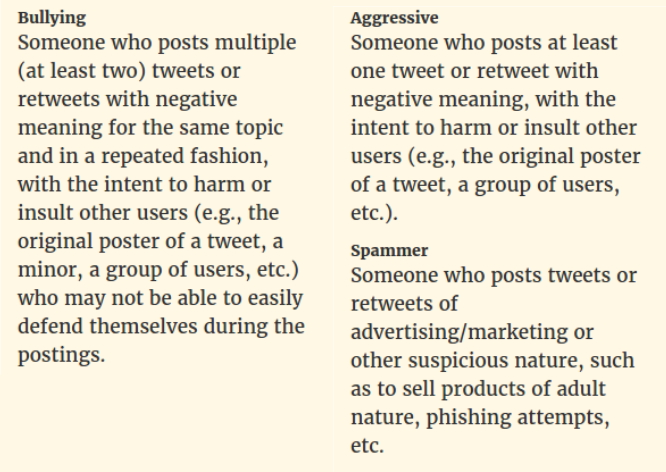
\includegraphics[width=0.47\textwidth]{img/twitter_defs}
\caption{Descriptions given to corwd sourcing workers in \cite{Twitter:2017}.}
\label{fig:twitter_defs}
\end{figure}

\subsubsection{Method}
\paragraph{Data} The data used by Chatzakou et al. is collected via Twitter's Streaming API\footnote{A service that offers free access to 1\% of all tweets (\url{https://dev.twitter.com/streaming/overview}).} between June and August 2016, resulting in a corpus of 1.65 million tweets (that is, the tweets themselves as well as metadata about the tweets and the users that sent them). More specifically, the corpus consists of two different sets. The \emph{baseline} (1 million tweets) is a set of random tweets. A \emph{hate-related} set (650K tweets) is gathered using 309 hashtags that are connected to bullying and hate speech. The set of hashtags is generated by using \#GamerGate as a start and collecting hashtags that appear alongside it.

The raw sets of tweets are furthermore processed in 3 steps. In a first step, the tweets are cleaned of noise by removing stop words, punctuation, numbers, URLs and emoticons. Also all characters are converted to lower case. Second, in order to remove spam, tweets from accounts with more than 5 hashtags per tweet on average as well as with an intra-tweet similarity above 0.8 are removed. Lastly tweets are grouped by user and into sessions\footnote{Where a session in defined as a consecutive set of tweets where no 2 tweets are seperated by 8 hours or more.} and those sessions furthermore split into batches of digestible size for labelling\footnote{The authors conclude through a preliminary experiment that batches with a size of 5-10 tweets are best suited for labelling.}. In this step users with fewer than 5 tweets in total and sessions with fewer than 5 tweets are removed. This results in 1,500 batches for each of the \emph{baseline} and \emph{hate-related} sets.

\paragraph{Labelling} For labelling the batches of tweets --- or rather, the users the batched tweets originate from, Chatzakou et al. employ 834 crowdsourcing workers on CrowdFlower\footnote{\url{https://www.crowdflower.com/}}. Each worker is given 10 batches of tweets and is only allowed to participate once. Furthermore, each batch is labelled by 5 workers. The possible labels are, as already mentioned, normal, aggressive, bullying and spammer. Through this method they receive a total of 1,307 annotated batches (9,484 tweets).

To evaluate the reliability of the crowdsourcing workers Cha\-tzakou et al. calculate the inter-rater agreement for the annotated batches with Fleiss's kappa, which turns out to be 0.54. Furthermore, they annotate 3 batches by themselves and include one of them into each of the 10 batch packages a worker receives. These control cases turn out to get labelled with an overall accuracy of 66.5\% (83.75\% for spam, 53.56\% for bully, 61.31\% fpr aggressive).

\paragraph{Feature extraction} The features used in \cite{Twitter:2017} can be categorized into user based, text based and network based. User based features include basic properties like the number of days since the user's account was created and the number of tweets, but also information derived from the generated sessions (see \emph{Data} section above), like the number of sessions and the average size of a user's sessions. Text based features include things like the number of hashtags and emoticons but also more complex features like word embedding averages obtained with word2vec\footnote{\url{https://code.google.com/archive/p/word2vec/}}, a sentiment score from SentiStrength\footnote{\url{http://sentistrength.wlv.ac.uk/}} and a hate score based on Hatebase\footnote{\url{https://www.hatebase.org/}}. Lastly, network based features are, among others, a popularity measure (follower friend ratio), the amount of reciprocity (extend of reciprocated follower connections) and several centrality scores.

For all the gathered features the authors highlight differences between the labelled users groups (normal, aggressive, bullying, spammer) and wether or not they are statistically significant or not. They find, for example, that aggressive and bully users have a tendency to use more hashtags than normal users.


\paragraph{Machine learning} For their experiments Chatzakou et al. try out using all as well as subsets of their features and test various probabilistic, tree-based and ensemble classifiers. Fruthermore they compare a classification into 4 classes (normal, aggressive, bullying, spammer) with a classification into 3 (normal, aggressive, bullying). As for the classification algorithm they achieve best results with a random forest tree-based classifier and report their results based on this.

\subsubsection{Results} Testing the usefulness of the features shows that 12 of the 30 features collected don't help in distinguishing between the users classes. These features, which include for example all session based statistics, the hate score and the closeness centrality, are excluded from the analysis. The features that were most useful for each of the two classes settings and their information gain are shown in Figure \ref{fig:twitter_features}.

\begin{figure}
\centering
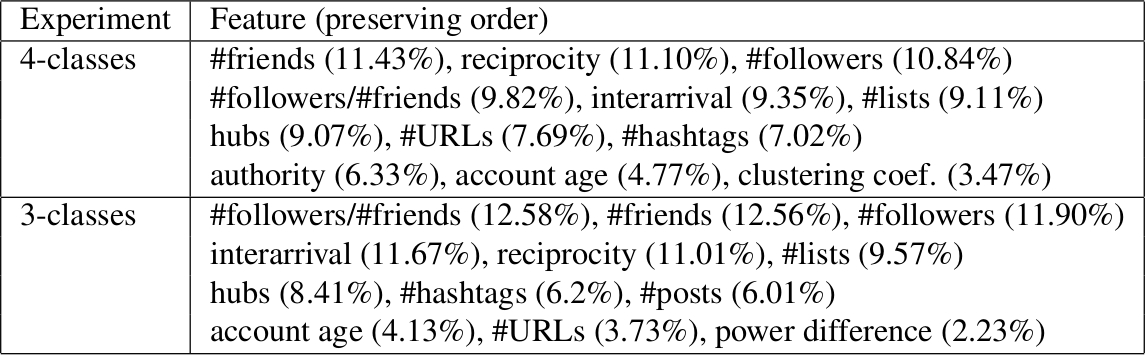
\includegraphics[width=0.47\textwidth]{img/twitter_features}
\caption{Feature evaluation in \cite{Twitter:2017}.}
\label{fig:twitter_features}
\end{figure}

In the 4 classes setting, the classification achieves an overall precision of 71.6\% and recall of 73.32\%. The 3 classes setting results in an average precision of 89.9\% and recall of 91.7\%, where the largest improvement can be seen for the bully class. Detailed results are shown in Figure \ref{fig:twitter_results}.

As an addition to their classification experiment based on tweets from June - August 2016, the authors examine the state of the labelled accounts in November 2016 and February 2017. They find that aggressive accounts got deleted by their users as well as suspended by Twitter to some extent, whereas none of the bully accouts as suspended but a larger percentage of them was deleted by the users themselves.

\begin{figure}
\centering
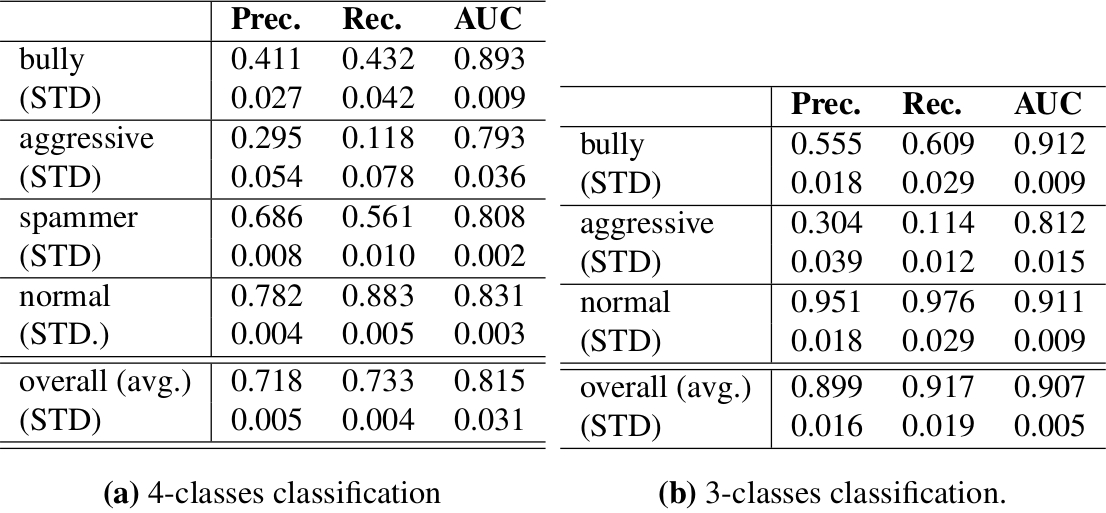
\includegraphics[width=0.47\textwidth]{img/twitter_results}
\caption{Classification results in \cite{Twitter:2017}.}
\label{fig:twitter_results}
\end{figure}

\subsubsection{Discussion} Chatzakou et al. test a wide range of properties of twitter accounts and their respective tweets. It is interesting to see that very few of the features connected to the actual texual content of tweets seems very useful for detecting abusive users. Or, put differently, that user and network features are much more informative. Maybe this is due to the short nature of tweets. Their preliminary experiment for establishing an optimal batch size for their crowdsourcing task shows an aspect of crowdsourcing that has to be thought of with care.

Since the paper makes no mention of language it could be assumed that only or mainly English tweets were used. However, with network and user features being the most useful it would be interesting to see if their appraoch works independent of language (i.e. is language agnostic).
%- batching: optimal batch size pre experiment nice\\

\subsection{Comparison}
- How do \cite{Yahoo:2016} and \cite{Twitter:2017} compare\\
\hphantom{- }- Classifying accounts (more features) vs. just comments\\
\hphantom{- }- Hate speech, derogatory language, profanity vs.\\
\hphantom{- - }bullying, aggression\\
\hphantom{- }- Ground truth: trained staff vs. crowd sourcing\\
\hphantom{- }- text based features useful vs. unuseful
- To what extend are they comparable

\section{Conclusion}
-

% \section{}
% \subsection{}
% \subsubsection{}
% \footnote{}
% \begin{math}\lim_{n\rightarrow \infty}x=0\end{math}
% \begin{equation}\lim_{n\rightarrow \infty}x=0\end{equation}
% \begin{displaymath}\sum_{i=0}^{\infty} x + 1\end{displaymath}
% \begin{table}
% \centering
% \caption{Frequency of Special Characters}
% \begin{tabular}{|c|c|l|} \hline
% Non-English or Math&Frequency&Comments\\ \hline
% \O & 1 in 1,000& For Swedish names\\ \hline
% $\pi$ & 1 in 5& Common in math\\ \hline
% \$ & 4 in 5 & Used in business\\ \hline
% $\Psi^2_1$ & 1 in 40,000& Unexplained usage\\
% \hline\end{tabular}
% \end{table}
%
% \begin{table*}
% \centering
% \caption{Some Typical Commands}
% \begin{tabular}{|c|c|l|} \hline
% Command&A Number&Comments\\ \hline
% \texttt{{\char'134}alignauthor} & 100& Author alignment\\ \hline
% \texttt{{\char'134}numberofauthors}& 200& Author enumeration\\ \hline
% \texttt{{\char'134}table}& 300 & For tables\\ \hline
% \texttt{{\char'134}table*}& 400& For wider tables\\ \hline\end{tabular}
% \end{table*}
%
% \begin{figure}
% \centering
% \epsfig{file=fly.eps}
% \caption{A sample black and white graphic (.eps format).}
% \end{figure}
%
% \newtheorem{theorem}{Theorem}
% \begin{theorem}
% Let $f$ be continuous on $[a,b]$.  If $G$ is
% an antiderivative for $f$ on $[a,b]$, then
% \begin{displaymath}\int^b_af(t)dt = G(b) - G(a).\end{displaymath}
% \end{theorem}
%
% \begin{figure*}
% \centering
% \epsfig{file=flies.eps}
% \caption{A sample black and white graphic (.eps format)
% that needs to span two columns of text.}
% \end{figure*}

\bibliographystyle{abbrv}
\bibliography{bibliography}  % bibliography.bib is the name of the Bibliography in this case

% remember to run:
% latex bibtex latex latex
% to resolve all references
%
% ACM needs 'a single self-contained file'!

\balancecolumns
\end{document}
